\chapter{NCC}
Please tell more about conclusion and how to the next work of this study.

\section{Lusia Violita Aprilian-1184080}
\subsection{Teori}
\begin{enumerate}
\item Menjelaskan kenapa file teks harus dilakukan tokenizer
	\par Tokenizer adalah untuk membuat vektor dari teks. Dan mengapa harus dilakukan tokenizer? itu karena dengan memfungsikan tokenizer, teks dapat divektorkan. Sehingga teks yang telah telah divektorkan tersebut dapat terbaca pada Machine Learning.
	\par Berikut adalah ilustrasi pemakaian pada tokenizer, perhatikan gambar \ref{7A1}:
		\begin{figure}[!hbtp]
		\centering
		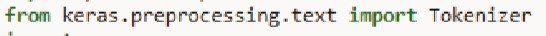
\includegraphics[scale=0.4]{figures/v1.jpg}
		\caption{Lusia-Tokenizer}
		\label{7A1}
		\end{figure}

\item Menjelaskan konsep dasar K-Fold Cross Validation
\item Menjelaskan kode program for train, test in splits.
\item Menjelaskan maksud kode program
\item Menjelaskan maksud fungsi
\item Menjelaskan maksud fungsi
\item Menjelaskan maksud fungsi
\item Menjelaskan maksud fungsi

\item Menjelaskan apa itu Deep Learning
	\par Deep Learning merupakan cabang dari Machine Learning atau bagian keluarga yang lebih luas dari method machine learning berdasarkan pada representasi data pembelajaran. Deep Learning menggunakan Deep Neural Network dalam menyelesaikan suatu masalah yang terjadi pada Machine Learning.

\item Menjelaskan apa itu Deep Neural dan bedanya dengan Deep Learning
	\par Deep Neural Network atau DNN merupakan algoritma yang berbasis neural network yang digunakan untuk mengambil keputusan.
	\par Yang membedakan Deep Learning dengan  Deep Neural Network (DNN) adalah DNN merupakan algoritma yang digunakan pada Deep Learning, sedangkan Deep Learning merupakan model yang menggunakan algoritma DNN.

\item Menjelaskan perhitungan algoritma konvolusi
\end{enumerate}